\appendix

\section{Bootstrap Slope Distribution}
\label{app:bootstrap}

\begin{figure}[h]
\centering
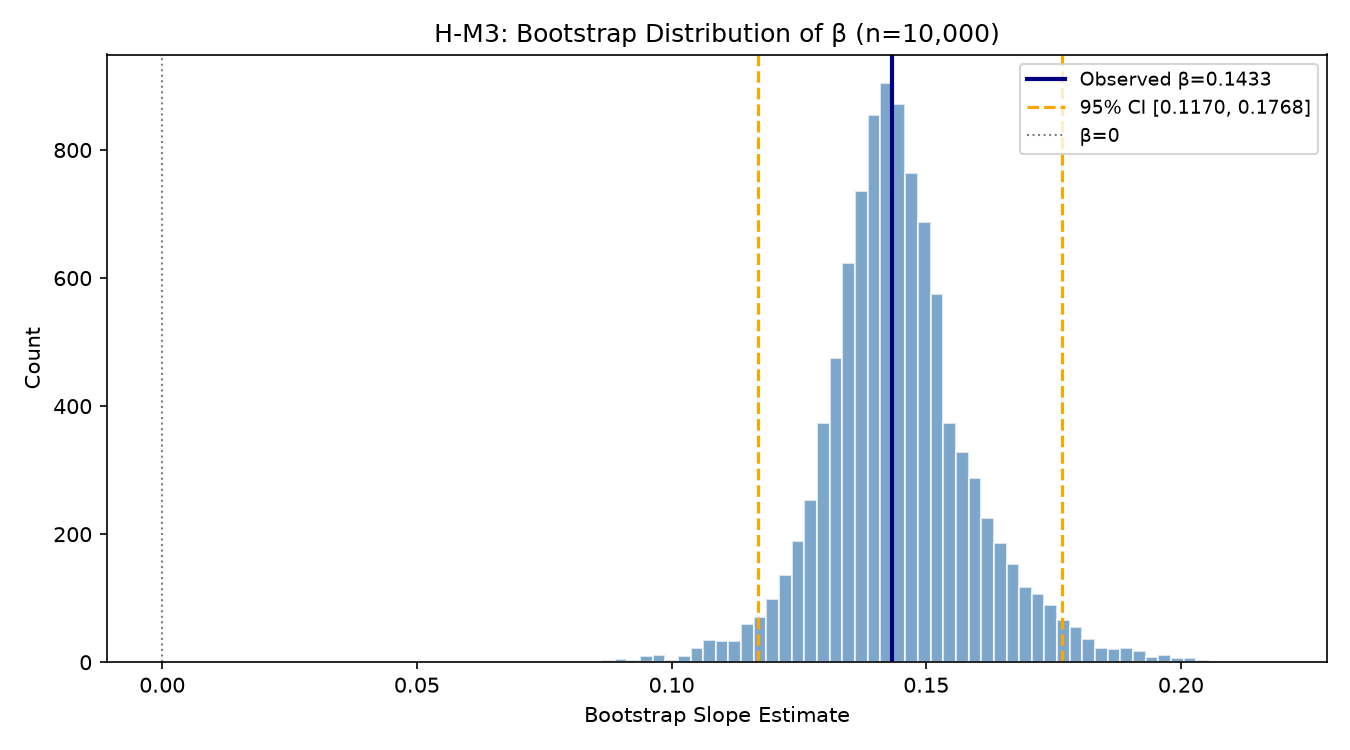
\includegraphics[width=0.7\columnwidth]{figures/bootstrap_histogram.png}
\caption{Bootstrap slope distribution for Coste et al.\ data ($N=10{,}000$ iterations, seed=42). The distribution is unimodal, approximately Gaussian, centered at $\beta \approx 0.143$, with bootstrap CI $[0.117, 0.177]$ strictly positive.}
\label{fig:bootstrap}
\end{figure}

\section{Gao et al.\ Dual-Axis Trajectory}
\label{app:gao}

\begin{figure}[h]
\centering
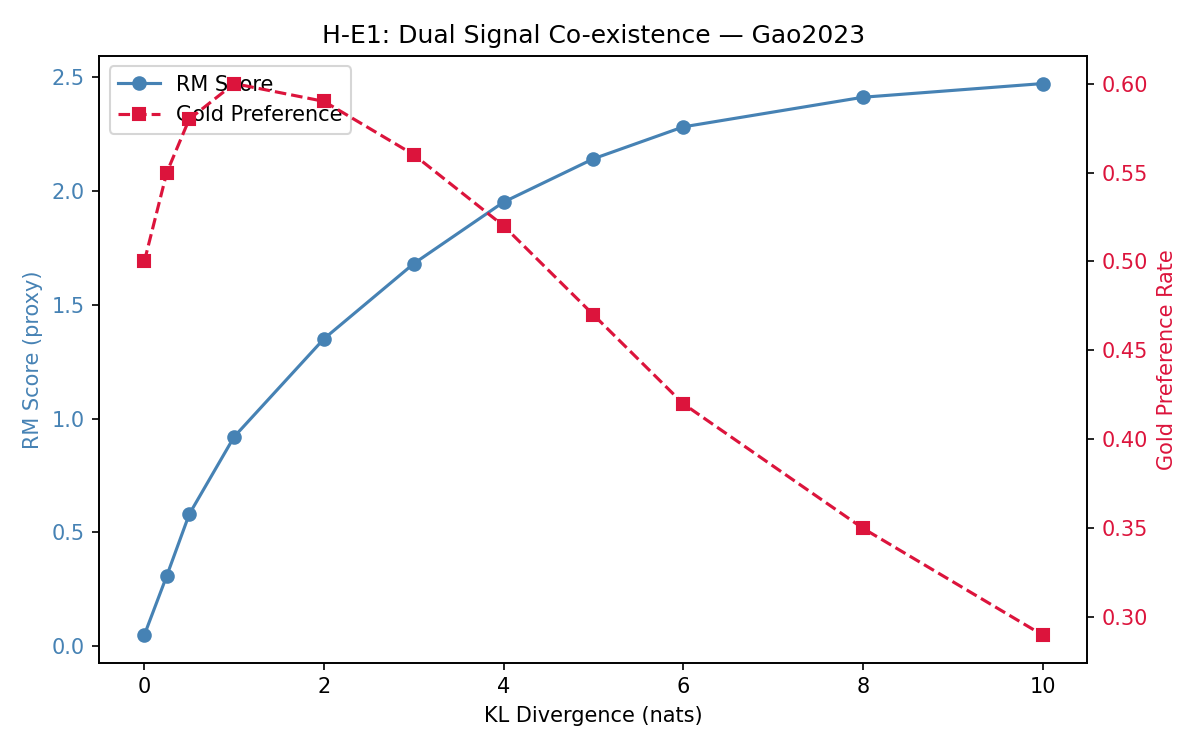
\includegraphics[width=0.7\columnwidth]{figures/dual_axis_gao2023.png}
\caption{Dual-axis plot for Gao et al.~\cite{Gao2023Scaling} across 11 KL checkpoints (all available levels, including the KL$=0$ boundary point used for signal characterization in H-E1). Unlike Coste data, the gap is initially negative at low KL (gold preference rises faster than RM), crosses zero at $\sim$3.5 nats, then enters the positive regime. This non-monotone shape accounts for the lower $R^2 = 0.701$ in the Gao linear regression, which uses $n=10$ observations (the KL$=0$ boundary point excluded; see Section~\ref{subsec:replication}).}
\label{fig:gao_dual}
\end{figure}

\section{Full Regression Summary (Coste et al.)}
\label{app:regression}

\begin{verbatim}
OLS Regression Results (statsmodels)
Dep. Variable:  gap           R-squared:  0.958
N:              10            Adj. R^2:   0.952
F-statistic:    181.2         Prob(F):    8.89e-07

Coefficients:
  const   -0.4016   (t = -8.344, p = 0.000)  [CI: -0.513, -0.291]
  KL       0.1433   (t = 13.461, p = 0.000)  [CI:  0.119,  0.168]

Omnibus: 1.751 (p=0.417)  Durbin-Watson: 0.411
Jarque-Bera: 0.868 (p=0.648)
\end{verbatim}
